% 3. A Condition--Driven Geometric Framework
\section{A Condition--Driven Geometric Framework}
We decompose any meshing method into six modules that translate \emph{conditions} into a \emph{geometric solution}:
\begin{enumerate}
  \item \textbf{Input} (data, problem definition): domain geometry and task specification.
  \item \textbf{Global Rule}: hard constraints that no method may violate (topological validity, non-overlap, boundary conformity, etc.).
  \item \textbf{Problem Reduction}: mapping the task to a simpler or already-solved problem (e.g., ``triangulate first, then convert to quads''). This step also detects conflicts between the problem definition and the global rules (infeasibility).
  \item \textbf{Local Rule}: algorithm-specific heuristics or policies (e.g., edge flips, front selection, templates).
  \item \textbf{Engine}: the driver that repeatedly applies rules to reach an \emph{objective} using a specific \emph{method} (incremental construction, global optimization, or physical relaxation).
  \item \textbf{Output}: the resulting mesh.
\end{enumerate}

Figure~\ref{fig:framework} summarizes the information flow.

\begin{figure}[t]
  \centering
  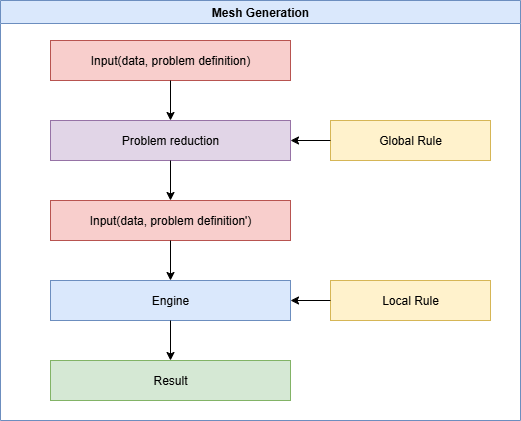
\includegraphics[width=0.9\linewidth]{figures/fw.png}
  \caption{The condition--driven framework: Input $\to$ Global Rule $\to$ Problem Reduction $\to$ (reduced Input) $\to$ Local Rule $\to$ Engine $\to$ Output.}
  \label{fig:framework}
\end{figure}

This lens foregrounds: (i) local vs global responsibilities; (ii) hard constraints vs soft preferences; and (iii) which modules are reusable infrastructure versus algorithm-specific policy. In the following sections we use this decomposition to remap historical families and extract design insights.
